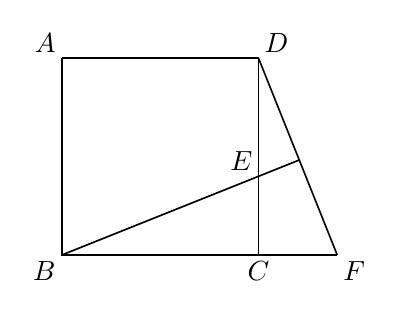
\begin{tikzpicture}[x=1cm,y=1cm,font=\normalsize,
 geometry edge/.style={solid,line width=.6pt},
 geometry mark/.style={solid,line width=.6pt},
 geometry label/.style={font=\normalsize,inner sep=2pt}]
\coordinate (A) at (0,2.5);
\coordinate (B) at (0,0);
\coordinate (C) at (2.5,0);
\coordinate (D) at (2.5,2.5);
\coordinate (E) at (2.5,1.0);
\coordinate (F) at (3.5,0);
\coordinate (G) at (3.0172,1.2069);
\draw[geometry edge] (A)--(B)--(F);
\draw[geometry edge] (C)--(D);
\draw[geometry edge] (A)--(D);
\draw[geometry edge] (D)--(F);
\draw[geometry edge] (B)--(G);
\node[geometry label,above left] at (A) {$A$};
\node[geometry label,below left] at (B) {$B$};
\node[geometry label,below] at (C) {$C$};
\node[geometry label,above right] at (D) {$D$};
\node[geometry label,above left] at (E) {$E$};
\node[geometry label,below right] at (F) {$F$};
\end{tikzpicture}
